\begin{figure}[htp]
	\centering
	\subfloat[Initial Noisy Data \newline
		\(\snr{x} = \SI{-4.68}{\dB}\)]
	{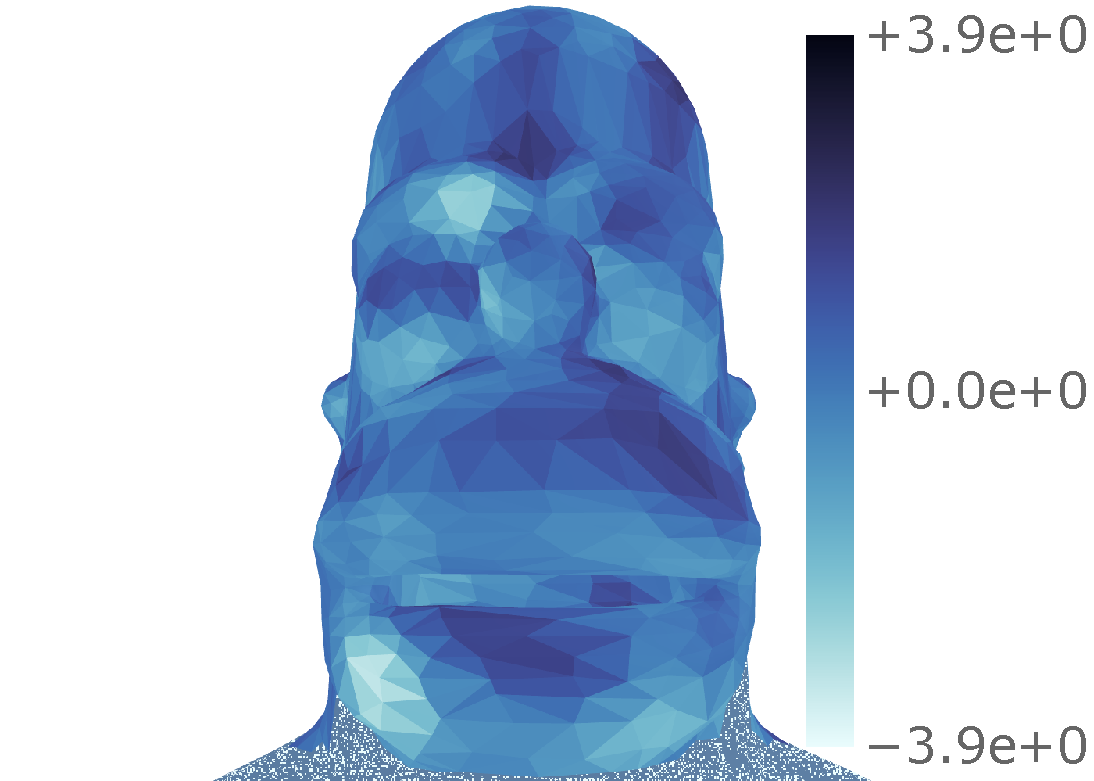
\includegraphics[trim={101 0 3 3},clip,width=.33\textwidth]{slepian_homer_field_-10noise_zoom.pdf}}
	\hfill
	\subfloat[Denoised \(N_{\sigma}=1\) \newline
		\(\snr{d} = \SI{-0.82}{\dB}\)]
	{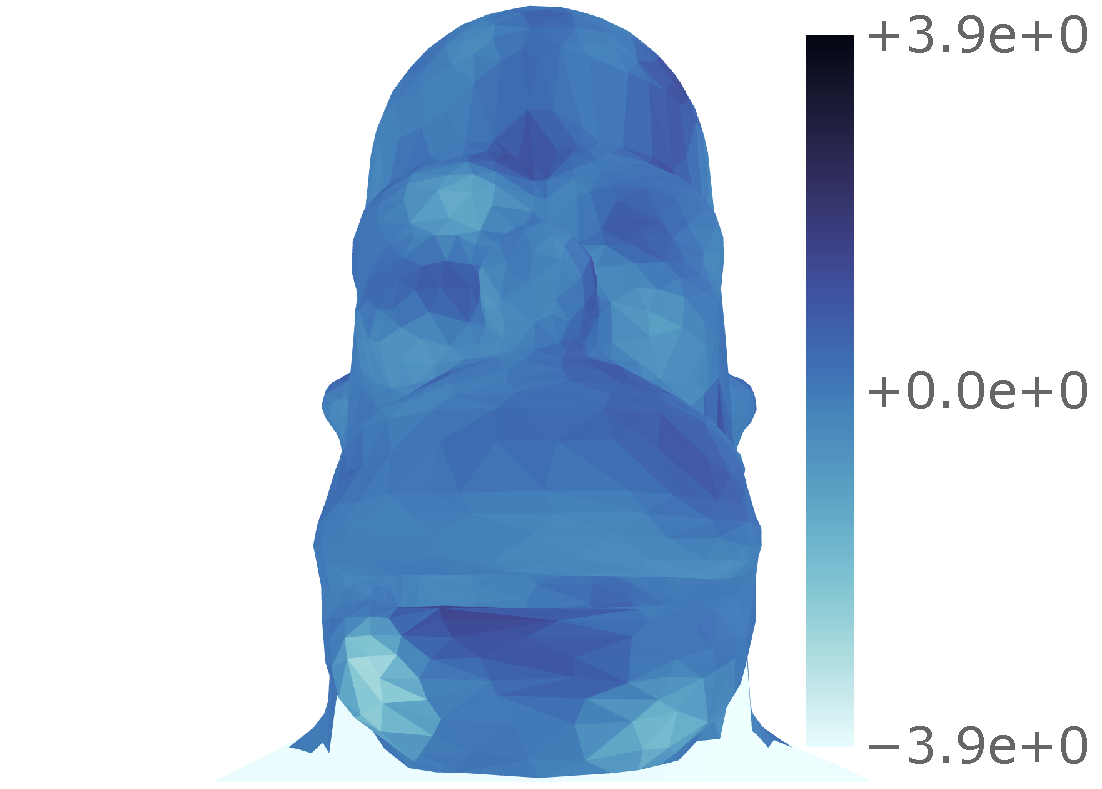
\includegraphics[trim={101 0 3 3},clip,width=.33\textwidth]{homer_-10snr_1n_denoised.pdf}}
	\hfill
	\subfloat[Denoised \(N_{\sigma}=2\) \newline
		\(\snr{d} = \SI{-0.08}{\dB}\)]
	{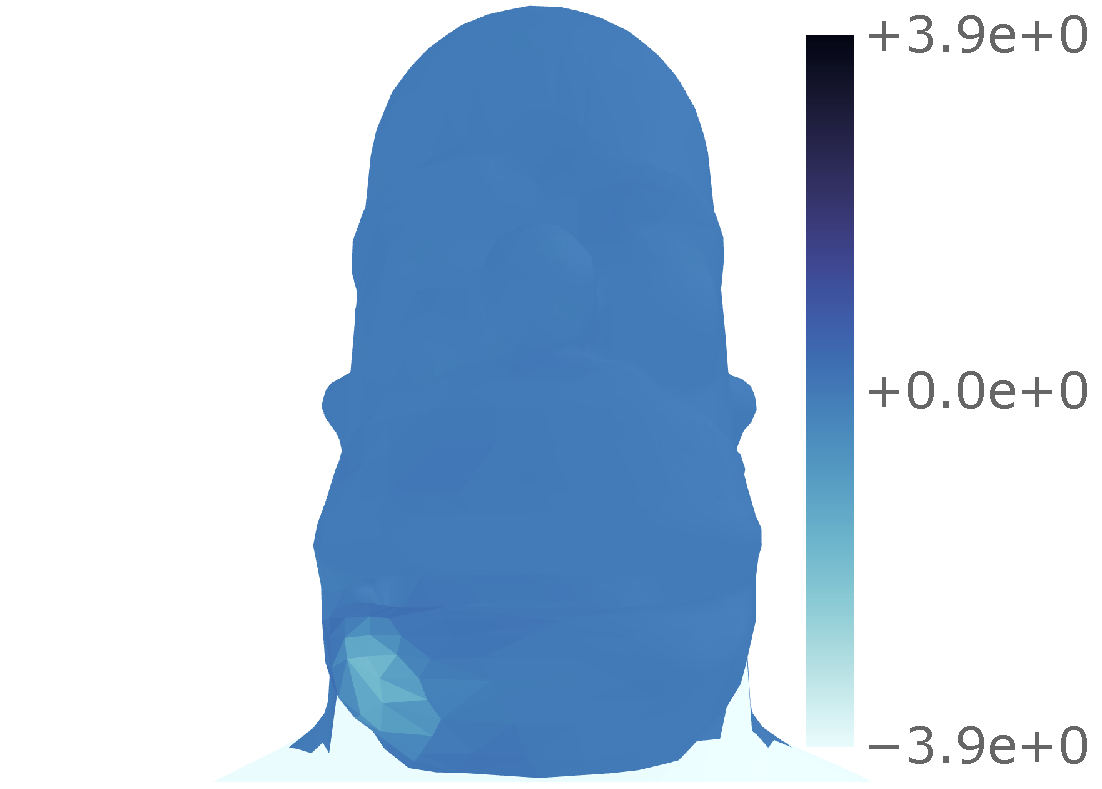
\includegraphics[trim={101 0 3 3},clip,width=.33\textwidth]{homer_-10snr_2n_denoised.pdf}}
	\caption{
	}\label{fig:chapter4_denoising}
\end{figure}
